\section{Frequency Filtration}
\label{sec:filtering}
The previous section provides motivation for finding ways to reduce both the
number of datapoints and the number of signals present in an \ac{FID} of
interest, without compromising the ability of the estimation routine
to parameterise it. A means of generating frequency-filtered ``sub-\acp{FID}''
is presented, which is able to achieve both of these. In essence, this
sub-\ac{FID} approach transforms the problem of \ac{FID} estimation from a
single large-scale estimation problem to a number of smaller-scale problems.
As well as realising vast improvements in computational speed, filtering also
enables a user to focus solely on spectral regions that are of interest.
It is common for certain spectral regions to be so densely populated
that it is futile to attempt to extract meaningful quantitative information at
the per-signal level, especially with \ac{1D} \ac{NMR} data. By applying
filtering, all focus can be devoted to those reasons which can realistically be
studied.

The concept of estimating selected regions in \ac{NMR} can be traced back to
Tang and Norris's \ac{LP}-ZOOM method\cite{Tang1988}, which employs the use of
\textit{subband decomposition}. A number of methods, including adaptive ones
in which the subbands employed for estimation are adjusted according to certain
criteria, have also emerged\note{add citations}.

\subsection{The \acl{VE}}
\label{subsec:ve}
The key steps of the filtering procedure used in this work consists of (i)
taking the \ac{FT} of the \ac{FID} (ii) applying a band-pass filter
to nullify parts not being considered, and (iii) returning the spectrum back to
the time-domain by an \ac{IFT}.
For a filtered sub-\ac{FID} to be faithfully modelled by a
summation of exponentially damped complex sinusoids, it is necessary that the
spectral peaks of interest lie effectively entirely within the filter
region\footnote{
    Lorentzian lineshapes tend to, but don't reach zero, as the distance from
    the maximum tends to $\infty$ (\cref{eq:lorentzian}). However, as long as a
    sufficiently wide filter region is defined, the ``tails'' of the Lorentzian
    which fall outside the filter window can be assumed to be negligible,
    especially when in the presence of noise.
}.
Due to their narrower linewidths relative to dispersion Lorentzians
(\cref{fn:lorentzian-decay}, \cpageref{fn:lorentzian-decay}), a spectrum solely
comprising absorption Lorentzians is therefore desired.
The \ac{VE} has been employed here, which has found application in the field of
compressed sensing NMR\cite{Mayzel2014,Golowicz2020,Luo2020}. The \ac{VE} is a
signal with double the size as the original \ac{FID}, with the key
characteristic that its \ac{FT} has a real component which is equivalent to its
counterpart derived from an unaltered \ac{FID} zero-filled to doubled its size,
and an imaginary component of zeros. The \ac{VE} concept can be applied
to data of any number of dimensions. However, only \ac{1D} virtual echoes are
employed in the work outlined in this thesis. An account of the \ac{2D} virtual
echo is provided in \cref{sec:multidim-ve}.

Assuming that a \ac{1D} \ac{FID} $\by \in \mathbb{C}^N$ is phased, such that
$\bdphi = \symbf{0} \in \mathbb{R}^M$, it can be described by
\begin{subequations}
    \begin{gather}
        y_n = \xi_n (c_n + \iu s_n) + w_n,\\
        \xi_n = \sum_m a_m \exp(-\eta_m n \Dt),\\
        c_n / s_n = \sum_m \cos / \sin(2 \pi f_m n \Dt).
    \end{gather}
\end{subequations}
The frequency-dependence has been decomposed into its real and imaginary
components. With this in mind, a conjugate pair of signals $\symbf{\psi}_{\pm}
\in \mathbb{C}^N$ are defined:
\begin{equation}
    \psi_{\pm,n} = \xi_n (c_n \pm \iu s_n) + w_n \equiv \Re(y_n) \pm \iu \Im(y_n)
\end{equation}
Two vectors $\symbf{t}_{1}, \symbf{t}_2 \in \mathbb{C}^{2N}$
are constructed using the conjugate pair.
$\symbf{t}_1$ is given by $\symbf{\psi}_+$ padded with zeros from below:
    \begin{equation}
        \symbf{t}_1 = \begin{bmatrix}
            \symbf{\psi}_+ \\ \symbf{0} \in \mathbb{C}^{N}
        \end{bmatrix}.
    \end{equation}
$\symbf{t}_2$ is given by $\symbf{\psi}_{-}$ with its elements in
    reversed order ($\cdot^{{\leftrightsquigarrow}}$), padded with zeros
    from above, and finally subjected to a right circular shift by one
    element ($\cdot^{{\circlearrowright}}$):
    \begin{equation}
        \symbf{t}_2 = \begin{bmatrix}
            \symbf{0} \in \mathbb{C}^{N} \\ \symbf{\psi}_-^{{\leftrightsquigarrow}}
    \end{bmatrix}^{{\circlearrowright}}.
   \end{equation}
The \ac{VE} $\by_{\text{ve}}$ is then given by $\symbf{t}_1 +
\symbf{t}_2$, with the first element divided by $2$, which is equivalent to
\begin{equation}
    \by_{\text{ve}} =
    \begin{bmatrix}
        \Re(y_0^{\vphantom{*}}) &
        y_1^{\vphantom{*}} &
        \cdots &
        y_{N-1}^{\vphantom{*}} &
        0 &
        y_{N-1}^* &
        \cdots &
        y_1^*
    \end{bmatrix}\T.
\end{equation}
As eluded to already, the \ac{FT} of $\by_{\text{ve}}$ produces a spectrum
$\symbf{s}_{\text{ve}}$ such that $\Im\left(\symbf{s}_{\text{ve}}\right) =
\symbf{0}$, with $\Re\left(\symbf{s}_{\text{ve}}\right)$ featuring absorption
Lorentzian peaks.

\subsection{The filtering process}
To filter the spectrum $\symbf{s}_{\text{ve}}$, it is subjected multiplication
with a function which acts as a band-pass filter. An example of a suitable
filter is a \emph{super-Gaussian} $\symbf{g} \in \mathbb{C}^{2N}$ defined by a
central index  $c \in \lbrace 0, \cdots, 2N-1 \rbrace$ and a bandwidth $b \in
\lbrace 0, \cdots, 2N-1 \rbrace$:
\begin{equation}
    g_n = \exp \left(-2^{p+1} \left(\frac{n - c}{b}\right)^p\right).
    \label{eq:super-Gaussian-onedim}
\end{equation}
The scalar $p \in \mathbb{R}_{>0}$ dictates the steepness
of the filter at the boundaries, with the function becoming more rectangular
as it increases. It is set to $40$ in this work. Application of the
super-Gaussian filter to $\symbf{s}_{\text{ve}}$
would lead to large sections of the filtered spectrum being $0$. This has an
undesired impact on the \ac{MDL}, as noise that resides within the filter
region will now seem to resemble true signal,
as its amplitude is infinitely greater than the zeroed regions. A massive
over-estimation of model order is likely to result because of this due to this.
In order to obtain better results from model order selection, an array of
synthetic \ac{AWGN} is
added to the filtered spectrum. To achieve this, a region in
$\symbf{s}_{\text{ve}}$ is specified which contains no discernible signal peaks
(referred to as the \emph{noise region}). The variance of this region
$\sigma^2$ is determined, and used to construct a vector of values sampled from
a normal distribution with mean $0$ and variance $\sigma^2$,
$\symbf{w}_{\sigma^2} \in \mathbb{R}^{2N}$.
The filtered spectrum is then given by
\begin{equation}
    \widetilde{\symbf{s}}_{\text{ve}} = \symbf{s}_{\text{ve}} \odot \symbf{g} + \symbf{w}_{\sigma^2} \odot \left(\symbf{1} - \symbf{g} \right).
    \label{eq:Sve-tilde}
\end{equation}
Note that the noise array's magnitude at each point is attenuated based on the
value of the super-Gaussian filter, as a means of ensuring the noise variance
remains consistent across the frequency space.

After filtering, $\widetilde{\symbf{s}}_{\text{ve}}$ is returned to the
time-domain by \ac{IFT}. The \ac{IFT} of a real-valued spectrum generates a
conjugate-symmetric signal, which is also a \ac{VE}. This is sliced so as to
retain the first half, which is the final filtered sub-FID $\widetilde{\by} \in
\mathbb{C}^{N}$.
A depiction of the key elements involved in the filtering process is provided
by \cref{fig:filtering}, while a step-by-step outline is provided by
\cref{alg:filter-1d}.
\begin{figure}
     \centering
     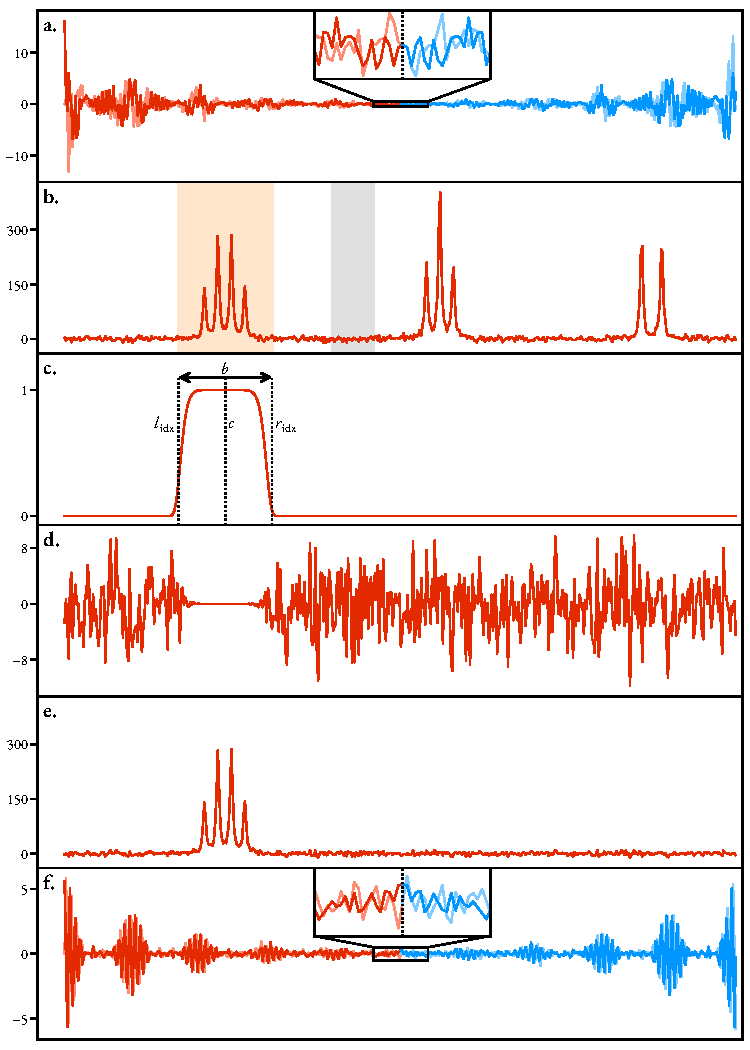
\includegraphics{filtering/filtering.pdf}
     \caption[
         An illustration of the filtering procedure applied to a \acs{1D}
         \acs{FID}.
     ]{
         An illustration of the filtering procedure applied to a \ac{1D}
         \ac{FID}.
         \textbf{a.} A \ac{VE} $\by_{\text{ve}}$, with the first and last
         $N$ points coloured red and blue, respectively. The middle of the
         \ac{VE} is magnified to highlight its conjugate symmetry.
         \textbf{b.} The \ac{FT} of the \ac{VE}, $\symbf{s}_{\text{ve}}$.
         The region of interest (orange) and noise region (grey) are denoted.
         \textbf{c.} A super-Gaussian function used as a band-pass filter,
         $\symbf{g}$.
         \textbf{d.} Synthetic noise vector to be added to the filtered
         spectrum, $\symbf{w}_{\sigma^2} (\symbf{1} - \symbf{g})$.
         \textbf{e.} The filtered spectrum $\widetilde{\symbf{s}}_{\text{ve}}$,
         formed by applying the super-Gaussian filter, and adding the noise
         vector.
         \textbf{f.} The \ac{IFT} of the filtered spectrum,
         $\widetilde{\symbf{y}}_{\text{ve}}$, from which the final filtered
         signal $\widetilde{\symbf{y}}$ is obtained by extracting
         the first $N$ (red) points.
     }
     \label{fig:filtering}
\end{figure}

The central index and bandwidth of the super-Gaussian filter function are given
by the following expressions:
\begin{subequations}
    \begin{gather}
        c = \tfrac{1}{2} \left(l_{\text{idx}} + r_{\text{idx}}\right), \\
        b = l_{\text{idx}} - r_{\text{idx}},
    \end{gather}
\end{subequations}
where $l_{\text{idx}}$ and $r_{\text{idx}}$ denote the desired
indices where the filter's left and right bounds are located, respectively.
Array indices can be obtained from the corresponding spectral frequencies
$f_{\unit{\hertz}}$ via
\begin{equation}
    \begin{gathered}
        f_{\text{idx}} =
            \left \lfloor
                \frac
                {
                    \left(2N - 1\right)
                    \left(\fsw + 2 \left(\foff - f_{\unit{\hertz}}\right) \right)
                }
                {2 \fsw}
            \right \rceil \\
        \forall f_{\unit{\hertz}} \in
            \left[\foff - \tfrac{1}{2} \fsw, \foff + \tfrac{1}{2} \fsw\right].
        \label{eq:fidx}
    \end{gathered}
\end{equation}
Alternatively, conversion from \unit{\partspermillion} to array indices can be
achieved by replacing  $f_{\unit{\hertz}}$ in \cref{eq:fidx} with
$f_{\unit{\partspermillion}} f_{\text{sfo}}$, where $f_{\text{sfo}}$ is the
transmitter frequency (\unit{\mega \hertz}) and $f_{\unit{\partspermillion}}$
is the frequency expressed as a chemical shift.

\subsubsection{Spectrum slicing}
Thus far, the method described is able to reduce the number of signals,
however the filtered sub-\ac{FID} still comprises the same number of points.
However, it is clear that there are a large number of points outside the region
of interest in $\widetilde{\symbf{s}}_{\text{ve}}$ that do not possess any
meaningful information. Discarding such points will then lead to a sub-\ac{FID}
with the same information about the signals of interest, but with far
fewer points. To achieve this, a slicing ratio is defined, $\chi \in
\mathbb{R}: \chi> 1$, which dictates the left and right indices at which the
spectrum should be sliced:
\begin{subequations}
    \begin{gather}
        l_{\text{slice}} =
        \begin{cases}
            c - \left \lfloor \frac{b \chi}{2} \right \rfloor &
            \text{if } \geq 0 \\
            0 & \text{otherwise}
        \end{cases} \\
        r_{\text{slice}} =
        \begin{cases}
            c + \left \lceil \frac{b \chi}{2} \right \rceil &
            \text{if } \leq 2N - 1 \\
            2N - 1 & \text{otherwise}
        \end{cases}
    \end{gather}
\end{subequations}
The filtered spectrum is then sliced accordingly:
\begin{equation}
    \mathbb{R}^{r_{\text{slice}} - l_{\text{slice}}} \ni
    \widetilde{\symbf{s}}_{\text{ve,slice}} =
    \widetilde{\symbf{s}}_{\text{ve}}[l_{\text{slice}} : r_{\text{slice}} + 1] \equiv
    \begin{bmatrix}
        \widetilde{s}_{\text{ve},\hspace*{1pt}l_{\text{slice}}} &
        \widetilde{s}_{\text{ve},\hspace*{1pt}l_{\text{slice}} + 1} &
        \cdots &
        \widetilde{s}_{\text{ve},\hspace*{1pt}r_{\text{slice}}} &
        \widetilde{s}_{\text{ve},\hspace*{1pt}r_{\text{slice}} + 1}
    \end{bmatrix}\T.
\end{equation}
Generation of the final sub-\ac{FID} is then achieved in a similar fashion to
before: by performing \ac{IFT}, and retaining the first half of the signal.
It is also necessary to scale the signal by the ratio of the number of points
in the sliced spectrum and it's unsliced counterpart, in order to ensure that
the amplitudes of each signal are unaffected:
\begin{subequations}
    \begin{gather}
        \widetilde{\by} =
            \frac{r_{\text{slice}} - l_{\text{slice}}}{2N}
            \IFT(\widetilde{\symbf{s}}_{\text{ve,slice}})
            [0 : N_{\text{slice}}],\\
            N_{\text{slice}} = \left \lfloor \frac{r_{\text{slice}} - l_{\text{slice}}}{2} \right \rfloor
    \end{gather}
\end{subequations}
The associated sweep width and transmitter offset of the \ac{FID} will have
been altered by this process, and in order to derive accurate frequencies and
damping factors for the sliced signal, it is necessary to determine these. The
corrected values can be computed using
\begin{subequations}
    \begin{gather}
        f_{\text{sw,slice}} = \frac{r_{\text{slice}} - l_{\text{slice}}}{2N - 1} \fsw\\
        f_{\text{off,slice}} = \foff + \frac{\fsw}{2} \left(
            1 - \frac{l_{\text{slice}} + r_{\text{slice}}}{2N - 1}
        \right)
    \end{gather}
\end{subequations}

\begin{algorithm}
    \begin{algorithmic}
        \caption[
            Filtering procedure for 1D data.
        ]
        {
            Filtering procedure for 1D data.
            $l_{\text{idx}}$ and $r_{\text{idx}}$ are indices of the left and
            right bounds of the region of interest.
            $l_{\text{idx,noise}}$ and $r_{\text{idx,noise}}$ are the analogous
            bounds for the noise region. All of these values should be $\in
            \lbrace 0, \cdots 2N - 1 \rbrace$.
            These would typically be provided in units of \unit{\hertz} or
            \unit{\partspermillion} by a user; conversion to indices can
            be carried out using \cref{eq:fidx}.
            \textsc{RandomSample} indicates taking a random sample from the
            given distribution.
        }
        \label{alg:filter-1d}
        \Procedure{Filter$1$D}{
            $\by \in \mathbb{C}^{N},
            l_{\text{idx}},
            r_{\text{idx}},
            l_{\text{idx,noise}},
            r_{\text{idx,noise}}
            $}
            \State $\by_{\text{ve}} \gets \textsc{VirtualEcho$1$D}\left(\by\right)$;
            \State $\symbf{s}_{\text{ve}} \gets \FT\left(\by_{\text{ve}}\right)$;
            \State $c_{\text{idx}} \gets \nicefrac{\left(l_{\text{idx}} + r_{\text{idx}}\right)}{2}$;
            \State $b_{\text{idx}} \gets r_{\text{idx}} - l_{\text{idx}}$;
            \State $\symbf{g} \gets \textsc{SuperGaussian$1$D}\left(2N, c_{\text{idx}}, b_{\text{idx}}\right)$;
            \State $\symbf{s}_{\text{noise}} \gets \symbf{s}_{\text{ve}} \left[
                l_{\text{idx,noise}} : r_{\text{idx,noise}} + 1
            \right]
            $;
            \State $\sigma^2 \gets \Var\left(\symbf{s}_{\text{noise}}\right)$;
            \State $\symbf{w}_{\sigma^2} \gets \symbf{0} \in \mathbb{R}^{2N}$;
            \For {$n = 0, \cdots, 2N - 1$}
            \State $w_{\sigma^2,n} \gets \textsc{RandomSample}\left(\mathcal{N}\left(0, \sigma^2\right)\right)$;
            \EndFor
            \State $\widetilde{\symbf{s}}_{\text{ve}} \gets \symbf{s}_{\text{ve}} \odot \symbf{g} + \symbf{w}_{\sigma^2} \odot \left(\symbf{1} - \symbf{g}\right)$;
            \State $\widetilde{\symbf{y}}_{\text{ve}} \gets \IFT \left( \widetilde{\symbf{s}}_{\text{ve}} \right)$;
            \State $\widetilde{\symbf{y}} \gets \widetilde{\symbf{y}}_{\text{ve}}[:N]$;
            \State \textbf{return} $\widetilde{\symbf{y}}$;
        \EndProcedure
        \Statex
        \Procedure{VirtualEcho$1$D}{$\by \in \mathbb{C}^N$}
            \State \textbf{return} $
            \begin{bmatrix}
                \Re(y_0^{\vphantom{*}}) & y_1^{\vphantom{*}} & \cdots & y_{N-1}^{\vphantom{*}} & 0 & y_{N-1}^* & \cdots & y_1^*
            \end{bmatrix}\T
            $
        \EndProcedure
        \Statex
        \Procedure{SuperGaussian$1$D}{$N \in \mathbb{N}, c_{\text{idx}}, b_{\text{idx}}$}
            \State $\symbf{g} \gets \symbf{0} \in \mathbb{R}^{N}$;
            \For {$n = 0, \cdots, N - 1$}
                \State $g_n \gets \exp\left(
                    -2^{41} \left(
                        \frac{n - c_{\text{idx}}}{b_{\text{idx}}}
                    \right)^{40}
                    \right)
                $;
                \Comment{$p$ in \cref{eq:super-Gaussian-onedim} has been set to 40.}
            \EndFor
            \State \textbf{return} $\symbf{g}$
        \EndProcedure
    \end{algorithmic}
\end{algorithm}
